 \documentclass[oneside,a4paper,12pt]{book}
%\pagestyle{headings}
\usepackage{enumitem}
\usepackage{listings}
\usepackage{filecontents}
\usepackage[english]{babel}
\usepackage{csvsimple}
\usepackage{xcolor}
\usepackage{graphicx}
%\usepackage{hyperref}
\usepackage{siunitx}
\usepackage{tikz} % To generate the plot from csv
\usepackage{pgfplots}
\usepackage{pgfplotstable}
\pgfplotsset{compat=1.8}
\usepackage{booktabs} % For \toprule, \midrule and \bottomrule
\usepackage{float}
\usepackage[T1]{fontenc}
\usepackage[utf8]{inputenc}
\pgfplotsset{compat=newest} % Allows to place the legend below plot
\usepgfplotslibrary{units} % Allows to enter the units nicely
\frontmatter
\sisetup{
	round-mode          = places,
	round-precision     = 2,
}

\input{preamble}
\lstdefinestyle{base}{
	emptylines=1,
	breaklines=true,
	escapeinside={\%*}{*)}, 
	basicstyle=\ttfamily\color{black},
	moredelim=**[is][\color{orange}]{@}{@},
	moredelim=**[is][\color{blue}]{"}{"},
	moredelim=**[is][\color{red}]{ç}{ç},
}
% A B S T R A C T
% % % % % % % % % % % % % % % % % % % % % % % % % % % % % % % % % %

\chapter*{\centering Abstract}
\begin{quotation}
\noindent 
For processing data, it is necessary for the computer to parse it into a readable format. The building of a parser requires a model of the grammar of the input. For many new programming language dialects and log files, these models are sometimes not available. For creating a model, the structure and grammar information must be inferred from the source code, which is a time consuming process. The goal of this project is to find structure of software code automatically \ho{you did not find structure but rather cluster similarly structured statements together}. We introduce in this thesis a clustering approach with k-means. Through different representations -numerical vectors inferred from the textual information of segments of the input- structural information should be exploited and assigned to different clusters according to their similarity.

For splitting the input into representation vectors, the smallest instance that can hold structure is found. These are then clustered using the k-means algorithm. This should help developers get a better overview of the data and in a perfect case, make them able to create parser rules for each cluster based on its nearest assigned statements.

The used approach has some promising results, assigning different patterns into different clusters. For measuring the performance of our representation methods, we calculate v-measure scores ranging from $0$ to $1$, with $1$ being a complete match. Out of 24 possible combination of representation, four representations achieved good results, having a v-measure score equal or higher than $0.66$ for Java and another 4 with satisfying results, having equal or better scores than $0.4$. The representation methods which do well on Java, also do a good job, clustering C\#, XML and ABACUS log files, but perform poorly on Brainfuck, with v-measure scores around $0$.

\ugh{Having the concept of clustering languages, the resulting clusters were used to calculate a precision value measuring the overlap of the clusters of a first language with the vector representations of a second language for classifying the degree of relation between them.}\ho{rephrase in a clearer way}
Unfortunately, our approach did not perform well, as it classified every language with the exception of XML, as very closely related.
\end{quotation}
\clearpage



% C O N T E N T S 
% % % % % % % % % % % % % % % % % % % % % % % % % % % % % % % % % % % % % % % %
\tableofcontents

\mainmatter
%%%%%%%%%%%%%%%%%%%%%%%%%%%%%%%%%%
%%%% NEW CHAPTER %%%%%%%%%%%%%%%%%%%%%
%%%%%%%%%%%%%%%%%%%%%%%%%%%%%%%%%%
\chapter{Introduction}
\label{cha:introduction}
\section{Motivation}
Writing software means reading software code \cite{latoza2006maintaining}. For developers it is crucial to understand the state of the system in order to carry out development and software evolution tasks. As a consequence, developers often use as much time reading and understanding the written code as actually writing new code. Analysis tools for integrated development environments can help developers understanding code and reduce time for assessing software code \cite{nierstrasz2012agile}. For such tools to be created, a software model of the the language the tool is built for, must exist in the form of a parser. For many dialects of programming language these models do not exists. Aside from programming languages, log files are a very important part of software applications. Many software applications do produce auxiliary text files as output. These log files are used in various ways, for example in debugging and profiling purposes. While generating log files is a very simple and straightforward process, the understanding of log files can be quite hard, as these can be very large files with complex structure \cite{valdman2001log}.  If a model of the grammar and the underlying structure does not exist, it is necessary to infer these properties from the source code. The inferring of a software model and the building of a custom parser is a complex task that can take several people several months to accomplish. In this bachelors project, we try to build a tool that can distinguish different pattern and structures automatically from software code or log files \cite{dubey2006inferring}.
\section{Goal and Focus}
The goal of this thesis is to develop a software tool that can atomically find structure in (unknown) software code or log files and generate different sets consisting of related pattern, so that a parser rule can be inferred. The process of creating the software tool is divided into three different sub-problems that had to be addressed:

\begin{enumerate}[ label=\textbf{\arabic*}.]
	
	\item \textbf{Statement creation.} Structure manifests itself in an ordered sequence of different tokens. For finding different patterns, the smallest statement had to be found which is able to hold structural information. In this thesis, we assume that carriage returns indicate the beginning of a new pattern. A statement is then split into tokens. Multiple tokens are either separated by blank spaces or by special characters and contain one or more character. Special characters are single character Tokens.


	\item \textbf{Representation and differentiation.} For algorithmically deciding and quantifying the difference between statements, a mathematical representation of the statements needs to be introduced. The approaches used in these methods, differ from creating a vector out of defining features, but instead focuses on the type of symbols used in a token.

	\item \textbf{Clustering.} A programming language consists of a finite number of different pattern that are used for describing software. These pattern are therefore used multiple times, only differing in the used variables and parameters. Patterns that are similar or differ only in the variables they contain must be filtered. Filtering is achieved through k-means clustering. Patterns should be clustered according to their similarity.
\end{enumerate}

To achieve a solution to these sub-problems, certain assumptions about the commonalities of languages and log files had to be made. We try to keep these assumptions as minimal as possible, so that a wide variety of programming languages and log files could be analysed:

\begin{itemize}
	\item A language consists of a finite number of patterns that differ only in used variables and parameters.
	\item Software code contains indents and carriage returns, as it is best practice for many programming languages amongst most developers, to make them more human readable.
\end{itemize}


\section{Related Work}
Recognizing Patterns is an easy task for humans, as we learn at a very young age to recognize patterns such as digits whether they are handwritten, machine printed, bold, italic or even rotated. Decision making relies on correctly interpreting the patterns of your surroundings \cite{jain2000statistical}. The same statements are also true for computers. For this reason, there is extensive research in supervised and unsupervised classification algorithms. This thesis applies techniques that are also used in many other fields such as Data Mining, Document Classification and even bioinformatics \cite{jain2000statistical}.

This thesis concentrates on unsupervised classification and uses the k-means algorithm as described in the lectures of Andrew Ng \cite{ngcs229} for assigning classifications to our code and log file contents.

In this thesis we use a numerical representation for the input data. Brenda S Baker introduces the idea of a numerical representation of software code to find duplicates in software code that differ only in the naming of the parameters \cite{baker1993theory}. Unfortunately, this idea relies on knowing fundamental structures of the language used. But nevertheless, this led to the idea, to not separate between a language set and a parameter set, but between different sets of tokens. In this thesis, the sets are words, numerals and punctuation.
\ho{First, related work should be a chapter of its own. Second, what you have here is not a related work section. You need to look at what other people did in the past to solve this problem. How is your work different from theirs? How is your work similar to theirs? How does your work fit in the big picture? \etc}

\section{Outline}
The rest of the thesis is structured as follows:

\textbf{chapter 2} introduces the components of StructureFinder and explains how the used methods work.

\textbf{chapter 3} describes the design of the StructureFinder and how the methods introduced in chapter 2 are integrated.

\textbf{chapter 4} uses experiments to gather information about the performance of our implemented approach and discusses those findings.

\textbf{chapter 5} concludes the work and discusses topics for future expanding StructureFinder.

\chapter{Methods}
\label{sec:methods}
In this chapter we describe in detail the used methods for creating and tokenizing the input data and put forward the different representations used in the created tool (subsequently also referred to as StructureFinder). In our context, a method is defined as a process, which transforms the input data and if replaced, would result in a different output of StructureFinder.

\section{Statements and Tokens}\label{sec:statements-and-tokens}
To be able to cluster our input data, which are lines of codes, it first needs to be processed into smaller instances that are comparable to each other. As mentioned in the introduction, we use in this project two instances of segmentation: Statements and tokens, where a statement is consisting of one or more tokens. A statement can be created in different ways. Because the main effort of this thesis lies in the structural clustering using the k-means algorithm, the creation of statements is simplified.

\textbf{A statement is a line of code.} Carriage retunes and line feeds are a very important way to make software code readable, creating a structure the human eye can perceive more easily. The way of using carriage returns and line feeds for defining a statement, tries to exploit the way we make software code and log files more readable for humans.



For visualising our methods, we introduce a simplified Java example.
In this example code, each new line becomes a statement, creating three different statements from this code snippet: 
\begin{center}
\begin{lstlisting}[caption=Statements in Java example, style = base,
	label=lst:java snippet,]
	@if (x > 1) {return 0;}@
	"if (x <= 0) {return 1;}"
	çelse {return v1;}ç
\end{lstlisting}
\end{center}
\textbf{A token is a single word, numeral or punctuation.} A statement is further processed into tokens, which are words, numerals, or punctuations.
\begin{itemize}
\item	A \textbf{Word} is a sequence of at least one letter and can contain numerals but cannot contain punctuation. 
\item A \textbf{Numeral} is a sequence of at least one digit. A numeral cannot contain letters or punctuation. 
\item A \textbf{Punctuation} is one special character which cannot be a letter nor a digit.
\end{itemize}
 
In our example tokens would be made as follows:

\begin{center}
\begin{lstlisting}[caption=Tokens in statements, style = base,
	label=tokens,]
	@if@ "("@x@ ">" ç1ç")" "{"@return@ ç0ç";""}" 
	@if@ "("@x@ "<""=" ç0ç")" "{"@return@ ç1ç";""}"
	@else@ "{"@return@ @v1@";""}"
	
\end{lstlisting}
\end{center}
In this example, the words are marked in orange, numerals are in red and punctuations are coloured blue. Tokens are divided by spaces. Punctuation that is not encapsulated by spaces will still be tokenized as an separate special characters. This means, as seen in the previous example that "$<=$" will be tokenized into two tokens: "$<$" and "$=$".  Variables such as "v1" are tokenized as a word.

\section{Representers}
\label{sec:reps}
As mentioned in the introduction, vector representation is needed for clustering statements. A representer calculates a vector representation out a statement or modifies already existing representations. There are three different categories of representers: Type representers, distance representers and weight representers.
\begin{enumerate}[ label=\textbf{\arabic*}.]
	
		\item \textbf{Type Representer} creates vector representations according to the characteristics of the tokens of the statement and assign numbers to the vector accordingly.
	
	
		\item \textbf{Distance Representer} calculates distance information from the given representation of a Type Representer.
	
		\item \textbf{Weight Representer} functions as a noise cancelling or filtering mechanism and can weight specific parts of a representation.

\end{enumerate}

Representers can be concatenated in the order shown above. A Type Representer is always needed, but can optionally be followed by a Distance Representer or a Weight Representer or both.

\subsection{Type Structure Representer}\label{sec:type-structure-representer}
The first Type Representer to be looked at, is the Type Structure Representer. It assigns a strict value according to the type of the token.\\\\
Example: In our implementation we assigned the values 0 for words, 1 for numerals and 2 for Punctuation. For our previous used Java snippet in Listing \ref{lst:java snippet}

\begin{lstlisting}[caption=Simplified Java snippet, style = base,
label=a_label,]
@if@ "("@x@ ">" ç1ç")" "{"@return@ ç0ç";}" 
@if@ "("@x@ "<=" ç0ç")" "{"@return@ ç1ç";}" 
@else@ "{"@return@ @v1@";}"    
\end{lstlisting}
Type Structure Representer gives us the vector representations:
\begin{lstlisting}[caption=Type Structure Representation example as vectors, style = base,
label=lst:type structure representation,]
(@0@ "2" @0@ "2" ç1ç "2 2" @0@ ç1ç "2 2")
(@0@ "2" @0@ "2 2" ç1ç "2 2" @0@ ç1ç "2 2")
(@0@ "2" @0 0@ "2 2")
\end{lstlisting}
\subsection{Type Specific Representer}
The Type Specific Representer uses the same structural information for calculating the vector representation as the Type Structure Representer. But instead of assigning a single value per type, the Type Specific Representer assigns a value per encountered unique token, with the exception of bracket symbols, for which opening and closing brackets are treated as one unique token.

To maintain the structural information of the statement, the assigned value per unique token is then normed into intervals, corresponding to the defined type values in subsection \ref{sec:type-structure-representer}.
An element of the vector representation is then calculated as follows:

\begin{centering}
	$\displaystyle \centering vector\_element = \frac{1}{assigned\_token\_value} + type\_value$\\
\end{centering}

with $vector\_element$ being the vector element of the representation at the position of the encountered token, $ assigend\_token\_value$ the value of the encountered token and $type\_value$ a predefined value for each different token type.

Example: Same as in the Type Structure Representer we assign the values 0 for words, 1 for numerals and 2 for Punctuation. A punctuation token therefore is always in the interval ${( 2,3 ]}$.
\newline \newline For our previous used Java snippet in Listing \ref{lst:java snippet},
\begin{lstlisting}[caption=Type Specific Representation example, style = base,
label=a_label,]
@if@ "("@x@ ">" ç1ç")" "{"@return@ ç0ç";}"
@if@ "("@x@ "<=" ç0ç")" "{"@return@ ç1ç";}"
@else@ "{"@return@ @v1@";}"
\end{lstlisting}
 this gives us the vector representations:
\begin{lstlisting}[caption=Type Specific Representation as vectors example, style = base,
label=a_label,]
(%*\textcolor{orange}{$\frac{1}{1}+0$} \textcolor{blue}{$\frac{1}{2}+2$}  \textcolor{orange}{$\frac{1}{3}+0$} \textcolor{blue}{$\frac{1}{4}+2$} \textcolor{red}{$\frac{1}{5}+1$} \textcolor{blue}{$\frac{1}{2}+2$} \textcolor{blue}{$\frac{1}{6}+2$} \textcolor{orange}{$\frac{1}{7}+0$} \textcolor{red}{$\frac{1}{8}+1$} \textcolor{blue}{$\frac{1}{9}+2$} \textcolor{blue}{$\frac{1}{6}+2$}*))
(%*\textcolor{orange}{$\frac{1}{1}+0$} \textcolor{blue}{$\frac{1}{2}+2$}  \textcolor{orange}{$\frac{1}{3}+0$} \textcolor{blue}{$\frac{1}{4}+2$} \textcolor{blue}{$\frac{1}{10}+2$} \textcolor{red}{$\frac{1}{8}+1$} \textcolor{blue}{$\frac{1}{2}+2$} \textcolor{blue}{$\frac{1}{6}+2$} \textcolor{orange}{$\frac{1}{7}+0$} \textcolor{red}{$\frac{1}{8}+2$} \textcolor{blue}{$\frac{1}{9}+2$} \textcolor{blue}{$\frac{1}{6}+2$}*))
(%*\textcolor{orange}{$\frac{1}{11}+0$}  \textcolor{blue}{$\frac{1}{6}+2$} \textcolor{orange}{$\frac{1}{7}+0$} \textcolor{orange}{$\frac{1}{12}+0$} \textcolor{blue}{$\frac{1}{9}+2$} \textcolor{blue}{$\frac{1}{6}+2$}*))
\end{lstlisting}

\subsection{Distance Zero Representer}
The Distance Zero Representer tries to exploit distance information of statement tokens. It measures the distances between the occurrences of the same values given by the used Type Representer. Measurement starts with zero as a new type value is first encountered. If the same type value is encountered after that, the new vector element will be the distance between the first encounter and the current position of the vector element.
Example: For simplifying the example, Type Structure Representer is used for assigning type values.
\begin{lstlisting}[caption=Type Representation as calculated in Listing \ref{lst:type structure representation}, style = base,
label=a,]
(@0@ "2" @0@ "2" ç1ç "2 2" @0@ ç1ç "2 2")
(@0@ "2" @0@ "2 2" ç1ç "2 2" @0@ ç1ç "2 2")
(@0@ "2" @0 0@ "2 2")
\end{lstlisting}
Applying Distance Zero Representation to the above Java snippet gives:

\begin{lstlisting}[caption=Distance Zero Representation of Type Structure Representation, style = base,
label=a,]
(@0@ "0" @2@ "2" ç0ç "4 5" @7@ ç4ç "8 9")
(@0@ "0" @2@ "2 3" ç0ç "5 6" @8@ ç4ç "9 10")
(@0@ "0" @2 3@ "3 4")
\end{lstlisting}
\subsection{Distance All Representer}
The Distance All Representer calculates the maximal distance between the same type values. Type values are given by a Type Representer. It then sets the maximum distance as the new value for replacing the type value.\\\\
Example: Type Structure Representer is used for assigning type values:

\begin{lstlisting}[caption=Type Representation as calculated in Listing \ref{lst:type structure representation}, style = base,
label=a,]
(@0@ "2" @0@ "2" ç1ç "2 2" @0@ ç1ç "2 2")
(@0@ "2" @0@ "2 2" ç1ç "2 2" @0@ ç1ç "2 2")
(@0@ "2" @0 0@ "2 2")
\end{lstlisting}
Applying Distance All Representer gives the following representations:

\begin{lstlisting}[caption=Distance All Representation vector representation example, style = base,
label=a,]
(@5@ "3" @5@ "3" ç4ç "3 3" @5@ ç4ç "3 3")
(@6@ "3" @6@ "3 3" ç4ç "3 3" @6@ ç4ç "3 3")
(@2@ "3" @2 2@ "3 3")
\end{lstlisting}

\subsection{Weight Summary Representer}
The Weight Summary Representer is used for reducing noise in the statements. Multiple subsequent occurrences of the same type values are summarized into one vector element of this type value.
Example: In the following example benefit of this technique can be seen in reducing the difference between statement 1 and statement 2:
\begin{lstlisting}[caption=Type Representation as calculated in Listing \ref{lst:type structure representation}, style = base,
label=a,]
(@0@ "2" @0@ "2" ç1ç "2 2" @0@ ç1ç "2 2")
(@0@ "2" @0@ "2 2" ç1ç "2 2" @0@ ç1ç "2 2")
(@0@ "2" @0 0@ "2 2")
\end{lstlisting}
Applying WeightSummaryRepresenter gives the following representations: 

\begin{lstlisting}[caption=Weight Summary Representation vector representation example, style = base,
label=a,]
(@0@ "2" @0@ "2" ç1ç "2" @0@ ç1ç "2")
(@0@ "2" @0@ "2" ç1ç "2" @0@ ç1ç "2")
(@0@ "2" @0@ "2")
\end{lstlisting}
\subsection{Weight Sum First Representer}
In code, important information such as keywords can often be found in the beginning of a line of code. Weight Sum First Representer adds all type values or distance values, following the current position, giving the vector elements in the beginning a higher weight.\newline
Example: For our previously used Java snippet in Listing \ref{lst:type structure representation}, applying Weight Sum First Representer gives the following representations. 
\begin{lstlisting}[caption=Weight Sum Representation vector representation example, style = base,
label=a,]
(@14@ "14" @12@ "12" ç10ç "9 7" @5@ ç5ç "4 2")
(@16@ "16" @14@ "14 12" ç10ç "9 7" @5@ ç5ç "4 2")
(@6@ "6" @4 4@ "2 2")
\end{lstlisting}

\subsection{Weight Inverse Representer}
The Weight Inverse Representer inverses every vector element. This reduces the variance of the data and inverses the weigh of the statement representation.
Example: The representation of the Type Structure Representer as shown in Listing \ref{lst:type structure representation} \ins{is }inverted. A Zero value, as possible in Type Structure Representation, is ignored in the calculation:
\begin{lstlisting}[caption=Type Specific Representation as vectors example, style = base,
label=a_label,]
(%*\textcolor{orange}{0} \textcolor{blue}{$\frac{1}{2}$}  \textcolor{orange}{$0$} \textcolor{blue}{$\frac{1}{2}$} \textcolor{red}{$\frac{1}{1}$} \textcolor{blue}{$\frac{1}{2}$} \textcolor{blue}{$\frac{1}{2}$} \textcolor{orange}{$0$} \textcolor{red}{$\frac{1}{1}$} \textcolor{blue}{$\frac{1}{2}$} \textcolor{blue}{$\frac{1}{2}$}*))
(%*\textcolor{orange}{$0$} \textcolor{blue}{$\frac{1}{2}$}  \textcolor{orange}{$0$} \textcolor{blue}{$\frac{1}{2}$} \textcolor{blue}{$\frac{1}{2}$} \textcolor{red}{$\frac{1}{1}$} \textcolor{blue}{$\frac{1}{2}$} \textcolor{blue}{$\frac{1}{2}$} \textcolor{orange}{$\frac{1}{1}$} \textcolor{red}{$\frac{1}{1}$} \textcolor{blue}{$\frac{1}{2}$} \textcolor{blue}{$\frac{1}{2}$}*))
(%*\textcolor{orange}{$0$}  \textcolor{blue}{$\frac{1}{2}$} \textcolor{orange}{$0$} \textcolor{orange}{$0$} \textcolor{blue}{$\frac{1}{2}$} \textcolor{blue}{$\frac{1}{2}$}*))
\end{lstlisting}
\section{K-Means}
K-means is an unsupervised clustering algorithm. It clusters the given data in k different clusters, with k being a known parameter, according to the vector representation of the data. For clustering the data, k different centroids are randomly initialized and the algorithm labels the data according to the nearest centroid. At the end of the algorithm, the centroids will have minimal distance to its assigned data points. This is achieved by moving the centroids to the euclidean mean of all the assigned data points. The mathematical expression, given the trainings set $\{x^{(1)},..., x^{(m)}\}$ and $x^{(i)} \in \mathbb{R}$ of the k-means algorithm is as follows:

\begin{figure}[H]
	\centering
	\includegraphics[width=0.8\textwidth]{kmeansformula}
	\caption{Mathematical expression of k-means \cite{ngcs229}.}
\end{figure}

A practical example of the k-means algorithm:\newline
	\begin{figure}[H]
		\centering
		\includegraphics[width=1\textwidth]{kmeansexample}
		\caption{Example of k-means iteration \cite{ngcs229}.}
	\end{figure}
The red and blue crosses visualize the centroids. They are initialized randomly at the start of the algorithm. The centroids will then in every iteration gradually move nearer to the mean of the final clusters, minimizing the cost of the distortion function:
\begin{center}
	$\displaystyle  J(c,\mu) = \sum_{i=1}^{m} ||x^{(i)} - \mu_{c^{(i)}}||^2$.
\end{center}
$J$ measures the sum of the squared distances between each training example $x^{(i)}$ and the centroid of the cluster $\mu_{c^{(i)}}$ to which it has been assigned.

\section{The Elbow Method}
\label{sec:elbow}
One problem of the k-means algorithm is that the parameter k must be known, which in our case is not known. K is dependent on the given input on which we want to limit our assumptions. Therefore, a way to algorithmically calculate k is needed. The idea behind the Elbow Method, is to find the number of centroids, so that if you add one centroid, the fit of the centroids to the data - measured by the cost function J-  does not improve significantly any more. In the case of k equals one, the position of the centroid would be the mean of all data points and in the case of k equals the number of all data points, the centroids would be the points themselves. As a consequence, k equals one results in the worst fit and while k equals the number of all data points gives perfect fit \cite{kodinariya2013review}. This can be illustrated by the following example where we normed J by k:

\begin{figure}[H]
	\begin{center}
		\begin{tikzpicture}
		\begin{axis}[
		width=\linewidth, % Scale the plot to \linewidth
		grid=major, % Display a grid
		grid style={dashed,gray!30}, % Set the style
		xlabel=k, % Set the labels
		ylabel= $ \frac{J(c,\mu ) }{ k} $,
		x unit=, % Set the respective units
		y unit=,
		legend style={at={(0.5,-0.2)},anchor=north}, % Put the legend below the plot
		%x tick label style={rotate=90,anchor=east}, % Display labels sideways
		y label style={rotate=-90}
		]
		\addplot 
		% add a plot from table; you select the columns by using the actual name in
		% the .csv file (on top)
			table[y=J/k,x=k,col sep=comma] {jbyk.csv}; 
				xmin=1,xmax =20,
		\legend{}
		\end{axis}
		\end{tikzpicture}
		\caption{Average Fit per centroid per k, calculated with StructureFinder using Java file input and TypeStructureRepresenter.}
	\end{center}
\end{figure}
As seen in the figure above, the improvement in the data modelling decreases as k becomes larger. By calculating the partial derivative $\displaystyle \frac{c_{i-1}-c_{i+1}}{k_{i-1} - k_{i+1}}$, the decrease can be measured. The partial derivative is maximized until it reaches a threshold $\alpha$, with $ \alpha \in \mathbb{R}^{^-}$. This value defines our guess for k.

\section{Language Differentiation}
\label{sec:langdiff}
Based on the representation based k-means clustering, this thesis also provides a method to calculate a precision value of how closely related two languages are. For this, one language is clustered with the k-means algorithm. For each cluster the radius is calculated ranging from the coordinate of the centroid to the assigned data point which is the furthest away from the centroid. For comparing a second language to the first, it suffices, to only calculate the vector representation of the data as discussed in section \ref{sec:reps}. For each represented data point of the second language, it is then checked, if it is inside any circle spanned from the previously calculated radii. The precision value describing the relation is calculated as follows:\newline
\begin{center}
	$\displaystyle \centering language\_relation =\frac{number\_of\_data\_points\_in\_radius}{number\_of\_data\_points} $
\end{center}

This means, that for any given two languages, the result $1$ indicates that the two languages are related closely and $0$ indicates that the languages are completely different. 
The two dimensional visualisation can be found in Figure \ref{fig:exLangDiff}. The red and blue crosses represent the data points of the clusters of the clustered language, with the centroid as the centre and the green crosses being the data points of the second language.
\begin{figure}[]
	\centering
	\includegraphics[width=0.7\textwidth]{circles.pdf}
	\caption{Two dimensional example of Language Differentiation}
	\label{fig:exLangDiff}
\end{figure}

In this example, only one of two green crosses, the data point of the second language, inside one of the two circles spanned from the radii of the previously calculated k-means clusterings blue and red. This would result in a precision value of $ \displaystyle\frac{1}{2}=0.5$.

\chapter{Implementation}
This chapter gives an overview of the implementation of the k-means clustering tool StructureFinder. First, we look at used resources. Second, that we look at the k-means and Language Differentiator pipeline and how the data is processed. 
\section{Technology}
StructureFinder is developed in Pharo 4.0 \cite{pharo2016}. Statements and tokens are separated with Petit Parser \cite{bergel2013deep}, which is also used for recognizing the types of the tokens.
\section{K-Means Pipeline}
\label{sec:kpipeline}
The first implementation to verify our ideas of clustering statements of software code was a simple k-means clustering algorithm with a single static k as a parameter.  
\newline\newline
\textbf{Known k.} The implementation of the k-means clustering  for calculating a single cluster is quite straightforward. A code file is loaded by a File Handler object. With the help of Petit Parser the loaded code file is then split into statements and tokens by the New Line Statementmaker. A Representer Runner is responsible for handling the different representation methods and calls to the loaded Representers. The Representers then successively create the vector representation. This representations get clustered by the implemented k-means algorithm. The processed clusters are then sent back to the File Handler, which saves each cluster in a separate file. Meaning it saves per centroid their assigned statements. The centroids are initialised in a range of values determined by the Representors used, so that no initialised value can be higher than any value of the calculated representations. This is done, to minimize the risk of getting centroids, without any data assigned to them, so called empty centroids.
The data flow can be seen in the following figure:
\begin{figure}[H]
	\centering
	\includegraphics[width=1\textwidth]{kmeans.pdf}
	\caption{Simplified data flow chart of the single k k-means pipeline.}
	\label{fig:kmeanspipeline}
\end{figure}

As discussed before, assumptions on the structure of the input should be minimal. Therefore we do not want to make assumptions about k, but want to have an algorithm to calculate the optimal number of clusters.

\textbf{Interval.} If the optimal number of clusters is not known, it is needed to calculate different clusterings with different numbers of clusters and compare them. For this, we implemented a way to create different clusters for a given interval. For each natural number in this interval, a set of clusters is calculated and then compared according to the elbow method discussed in section \ref{sec:elbow}. Each calculated set of clusters is given to the File Handler and output is created for each set of clusters in the same way as in the implementation shown above. All results from the distortion function, as well as the used representation and the optimal value of k is saved in a log file. The expansion results in this updated data flow:
\begin{figure}[H]
	\centering
	\includegraphics[width=1\textwidth]{bestkmeans.pdf}
	\caption{Simplified data flow chart of the expanded k-means pipeline, with highlighted differences to \ref{fig:kmeanspipeline} in yellow.}
	\label{fig:bestkmens}
\end{figure}

The Square Sum Analyser calculates the distortion function for the elbow method for guessing k for the different k-means clusterings.

For the updated implementation of StructureFinder, there is also a very important addition to the output: the nearest statements of the centroids of the best clustering. These statements are also saved to the log file. The bigger our input files are, the bigger the output files get. This makes it harder to get an overview of found structures based on lists of all the statements. The nearest statements of the centroids serve as perfect example and should incorporate the pattern featured in the corresponding centroid.


\section{Language Differentiation Pipeline}
As discussed in section \ref{sec:langdiff}, it is possible to use the implementation of the k-means clustering to calculate a precision value, measuring how closely related different languages are. The implementation is expanded by adding a control object for the language differentiation. The data flow of the Language Differentiation looks accordingly:
\begin{figure}[H]
	\centering
	\includegraphics[width=1\textwidth]{langdiffpipeline.pdf}
	\caption{Simplified data flow chart of the Language Differentiator pipeline.}
	\label{fig:langdiff}
\end{figure}
\section{Execution Time}
The execution time of StructureFinder is dependent on different parameters of the input and configuration.
The parameters the tool depends on, are the number of iterations, the size of the training data, the number of clusters, as well as the number of attributes, meaning the length of the vector representations.

While running the algorithm, we experienced significant slow downs for calculating the clusterings, using the Type Structure Representer or with calculation using the Weight Inverse Representer. These two representations are the only ones using float calculation, instead of integer calculations. Because there is a lot of vector calculation involved, it leads to the conclusion that floating point calculation is the cause of the slowdowns.
\section{Testing}
Testing is done in SUnit, which is integrated in Pharo 4.0. A test suite was implemented testing vector calculations and the correct functioning of the creation of the representation.
 
\chapter{Evaluation}
In this chapter, we evaluate how well the ideas we implement in this thesis work. For this, we first need to introduce a way to measure the performance of k-means clusterings and take a look how the elbow method should be configured. Second, we try to answer the question of which representation introduced in section \ref{sec:reps} performs the best. Third, we run StructureFinder on different languages to see, if it can handle different structural concepts and last, we look at how the clusters created from StructureFinder look like and what we can learn about the structure of input data out of its clustering.
After the evaluation of StructureFinder, we look shortly at the performance of our expansion for classifying the degree of relation between two languages.
\section{Evaluation Setup}
Evaluating an unsupervised learning algorithm does have the problem that there is no labelled data to test against. But since we know what the goal of the algorithm is supposed to be, we are able to manually cluster files into a reference clustering, making the cluster assignment ourselves to test our methods against. In a first paragraph, we can then introduce v-measures for calculating a score based on a reference clustering.
For calculating clusters we need to have a elbow threshold parameter $\alpha$ (introduced in section \ref{sec:elbow}) for guessing k, as we do not want to define k. So in a second paragraph we experimentally look for a desirable value of $\alpha$ for further computations.


\subsection{V-Measures}\label{sec:v-measures}
Given the knowledge of the ground truth class assignments of the samples, which we manually created, it is possible to define a metric, using conditional entropy analysis.\\\
In particular Rosenberg and Hirschberg \cite{rosenberg2007v} define the following two desirable objectives for any cluster assignment:
\begin{itemize}
	\item \textbf{homogeneity:} each cluster contains only members of a single class.
	\item \textbf{completeness:} all members of a given class are assigned to the same cluster.
\end{itemize}
Homogeneity and completeness scores are formally given by:\\\\

\begin{centering}
	$\displaystyle h = 1-\frac{H(C|K)}{H(C)}$ \\
\end{centering}
\begin{centering}
	$\displaystyle c = 1-\frac{H(K|C)}{H(K)}$\\
\end{centering}

with the conditional entropy of the classes, given the cluster assignments $H(C|K)$ being defined as:\\

\begin{centering}	$\displaystyle H(C|K) = -\sum_{c=1}^{|C|}\sum_{k=1}^{|K|}\frac{n_{c,k}}{n}log \Big( \frac{n_{c,k}}{n_k} \Big)$\\
\end{centering}

and the conditional entropy of the classes is given by:\\

\begin{centering}	
	$\displaystyle H(C) = -\sum_{c=1}^{|C|}\frac{n_{c}}{n}log \Big( \frac{n_{c}}{n} \Big)$\\
\end{centering}

where $n_k$ is the number of samples in cluster k and $n_{c,k}$ is the number of samples from class c assigned to cluster k.\\
The conditional entropy of clusters given class $H(K|C)$ and the entropy of clusters $H(K)$ are defined in a symmetric manner.\\\\
The V-Measure is defined as the harmonic mean of homogeneity and completeness:\\

\begin{centering}	
	$\displaystyle v = 2\frac{h*c}{h+c}$\\
\end{centering}
This gives us values for h, c and v ranging from $[0,1]$. These values can be used as a score to compare how well our representations performed, with 1 being a perfect score and 0 being the lowest score \cite{rosenberg2007v}.

\subsection{The Elbow Method}
The elbow method, as seen in Section \ref{sec:elbow}, is a heuristic for finding a good value for the parameter k. In our manually clustered Java data, we were able to cluster it into $13$ different clusters, making this our desired output of the elbow method. For the Type Structure and the Type Specific Representer we run the elbow methods with different threshold parameter $\alpha$ on Java the previously mentioned Java code file:

\begin{figure}[H]
	\begin{center}
		\begin{tikzpicture}
		\begin{axis}[
		width=1\textwidth, % Scale the plot to \linewidth
		grid=major, % Display a grid
		grid style={dashed,gray!30}, % Set the style
		xlabel=$\displaystyle \alpha$, % Set the labels
		ylabel= $\displaystyle k$,
		x unit=, % Set the respective units
		y unit=,
		%legend style={at={(0.5,-0.2)},anchor=north}, % Put the legend below the plot
		%x tick label style={rotate=90,anchor=east}, % Display labels sideways
		y label style={rotate=-90}
		]
		\addplot[color=red,mark=x]
		table[y=k1,x=alpha,col sep=comma] {kalpha.csv};
		% add a plot from table; you select the columns by using the actual name in
		% the .csv file (on top)
		
		\addplot[color=blue,mark=*]
		table[y=k2,x=alpha,col sep=comma] {kalpha.csv};
		%\addplot[color =green, mark =-]{13};
		\legend{Type Structure, Type Specific}
		\end{axis}
		\end{tikzpicture}
		\caption{Plot of elbow method. Heuristic value of k, given $\alpha$.}
	\end{center}
\end{figure}
The smaller $\alpha$, the smaller is k. These two plots show, that a value of $-3$ is needed to get near the desired value for k. Therefore $-3$ will be used for further calculations. It is important to notice that the calculated k differs for the same value of $\alpha$ for the two different used representation methods. Also we have to address the problem of statistical outliers, as can be seen in this graph at around $\alpha = -0.5$. Given that the underlying k-means algorithm is statistical, outliers are to be expected. Problems related to the k-means implementation are discussed in section \ref{sec:eval_kmeans}.

\section{Evaluating the Representations}
\label{sec:eval_kmeans}
Representations are an important part of StructureFinder, because they change the behaviour of the k-means algorithm. For further evaluation we want to know, which Representers perform well and should therefore be used if a new language is clustered. 


\subsection{V-Measure scores for Java}\label{sec:v-measure-scores-for-java}
Using the v-measure scores, we can calculate two tables containing all the possible representations introduced in this thesis. Table \ref{tab:measure-strcuture} is clustered using the Type Structure representation, while table \ref{tab:measure-sec} is calculated using Type Specific representation. The two tables are hierarchically structured. All the calculations in the two tables were made with clusterings for $k \in [10,25]$ and with the elbow threshold parameter $\alpha = -3$. Aside from the calculations of the scores for homogeneity, completeness and v-measures, the tables also feature the elbowed value for k as "perfect k". Using k-means clustering, it is possible for centroids to not be assigned to any data points. Because of this, the number of empty centroids encountered in the clustering is featured as well. While computing the v-measure scores, there was a problem with the range of the values computed. Under the condition of empty centroids present, there was a possibility for the scores to be below zero. Fortunately this was only the case if there were many centroids without assigned data points. For simplicity, these values were rounded to zero.

\begin{table}[H]
	\begin{center}
		\caption{Java v-measures of all possible representations with Type Structure Representer}
		\label{tab:measure-strcuture}
		
			\pgfplotstabletypeset[
			%trim cells,
			%multicolumn names, % allows to have multicolumn names
			col sep=semicolon, % the seperator in our .csv file
			read comma as period=true,
			%column type=1,
			every head row/.style={%
				before row=\toprule,
				after row=\midrule,
				typeset cell/.code={
					\ifnum\pgfplotstablecol=\pgfplotstablecols
					\pgfkeyssetvalue{/pgfplots/table/@cell content}{\multicolumn{1}{c}{##1}\\}%
					\else
					\pgfkeyssetvalue{/pgfplots/table/@cell content}{\multicolumn{1}{c}{##1}&}%
					\fi
				}
			},
			every last row/.style={after row=\bottomrule},
		display columns/0/.style={string type,column type={l}},
		display columns/1/.style={string type},
		display columns/2/.style={string type},
		display columns/3/.style={string type},
		display columns/4/.style={string type},
		display columns/5/.style={string type},
		]{results.csv} % filename/path to file
	\end{center}
\end{table}


\begin{table}[H]
	\begin{center}
		\caption{Java v-measures of all possible representations with Type Specific Representer}
		\label{tab:measure-sec}
		\pgfplotstabletypeset[
		%trim cells,
		%multicolumn names, % allows to have multicolumn names
		col sep=semicolon, % the seperator in our .csv file
		read comma as period=true,
		%column type=1,
		every head row/.style={%
			before row=\toprule,
			after row=\midrule,
			typeset cell/.code={
				\ifnum\pgfplotstablecol=\pgfplotstablecols
				\pgfkeyssetvalue{/pgfplots/table/@cell content}{\multicolumn{1}{c}{##1}\\}%
				\else
				\pgfkeyssetvalue{/pgfplots/table/@cell content}{\multicolumn{1}{c}{##1}&}%
				\fi
			}
		},
		every last row/.style={after row=\bottomrule},
		display columns/0/.style={string type,column type={l}},
		display columns/1/.style={string type},
		display columns/2/.style={string type},
		display columns/3/.style={string type},
		display columns/4/.style={string type},
		display columns/5/.style={string type},
		]{specificres.csv} % filename/path to file
	\end{center}
\end{table}
The best results were achieved by using only the two Type Representers. They scored extremely well in completeness with values up to $0.91$, if used without any other representation. The best scores however were achieved by adding the Weight Summary Representer, which as discussed in section \ref{sec:reps}, reduces noise in the type representation. With the addition of Weight Summary representation, the algorithm scores up to $0.95$ in completeness and works extremely well if used  with the Type Specific representation, but not as good with the Type Structure representation. If we look at the highest scores, Type Structure Representation is the better choice having both the highest score with the representation that uses only Type Representation and the highest score overall with the use of Type Specific Representation and the Weight Summary Representer. We will for further evaluation concentrate on the Type Representors and the Weight Summary Representor and will take a look on how they can cluster different languages. 

The heuristic guess for k does extremely well. As mentioned before, $\alpha = -3$ was used for the calculations of the elbow method. Of Interest are all the combination of Representers that do not result in empty centroids. For those representations, the guessed k varies maximally by 2 from the manually created example. For the best combination, being composed of the Type Specific and the Weight Summary, it only differs by one additional cluster.



\subsection{Discussion}\label{sec:explaining-the-results}

While there are pretty good results from StructureFinder, most of them have only low scores. This section tries to find an explanation, as to why.

\textbf{Assumptions.} The main goal of this thesis was to find structural patterns in software code files or log files, while keeping the assumptions about the structure of the input files as minimal as possible. One of the problems of using a clustering algorithm is, that said algorithm does make assumptions about the data it clusters. For k-means, this assumption lies in the goal of the algorithm to minimize the squared sum of the distances from the data points to the centroids. This might that it always tries to find clusters that are circular in shape. This might not be the case for the representations we create in this thesis, as the representations were created as seen fit for representing certain characteristics of structures in a statement.

\textbf{Variance.} If we look at the scores tables \ref{tab:measure-strcuture} and \ref{tab:measure-sec} , it is striking that methods do poor which allow for high variance in the representations. This is the case for all the Distance Representers, as well as for representations such as Weight Sum First. It is interesting to see, that the Distance Representers do better, if we lower the variance of the data, which is the case, if we additionally use the Weight Inverse Representer. This could be the case, again, because the k-means algorithm tries to minimize the squared sum distances from data points to centroids. With a big variance in the data, this can cause the k-means algorithm to give more weight to clusters that are more dense and thus neglecting smaller clusters with lower density \cite{rob2016k}.

\textbf{Empty Centroid.} In the results, we needed to feature a column for empty centroids, as this is a big problem that needs to be addressed. Centroids are randomly initialized with uniform distribution over all dimensions of the vector, scaled to the highest vector element found in the data. In contrast to featurization, representations allow for vectors of different sizes. For vector calculations this means that smaller vectors need to be padded with zeros to compare them. Therefore, more relevant data lies in the lower dimensions of a vector. If the centroids are uniformly initialised in every dimension, initialized centroids can be further away from the data points as any other centroid. We can see this in Weight Sum First, were we have high values at the beginning and low values at the end. So Weight Sum First increases this phenomena, but every method that allows for hight variance in the representation is therefore more prone to have empty centroids.

\textbf{Convergence.} Scores rely on the convergence of the k-means algorithm. For the algorithm to be guaranteed to converge to the optimal result, certain assumptions of the data must be met. If these assumptions are not met, it is possible that the algorithm converges to a local instead of a global optimum. In our thesis, it is unfortunately the case that these assumptions are not always met. This can result in different results, as in the tables above. This does not necessarily mean that our calculated data is not valid. If the Representers are run multiple times, the algorithm that did well in the scores, were actually the most robust ones, having the lowest variance in the scores and the distortion function. This can be traced back to the robustness in relation to the empty centroids, meaning, that if a representation is more likely to have empty centroids, it is also to be expected to have higher variance of the v-measures and in the distortion function.

\textbf{Summary.} The best representations in our evaluation were clearly the Type Structure and the Type Specific. It seems that they best fit in the assumptions made by the k-means algorithm and that their limited variance prevents them from suffering from empty centroids. For clustering new languages one of these two representation are likely to achieve satisfying results. For creating new representation methods the discussed topics above should be taken into account.

\subsection{Type Structure vs. Type Specific}\label{sec:type-structure-vs-type-specific}
The two Type Representers are performing reasonably well. In this section we want to find out, which of the two is expected to perform better. For this we use data calculated for the evaluation of the applicability for other languages in section \ref{sec:evaluating-other-languages}.

\definecolor{bblue}{HTML}{4F81BD}
\definecolor{rred}{HTML}{C0504D}
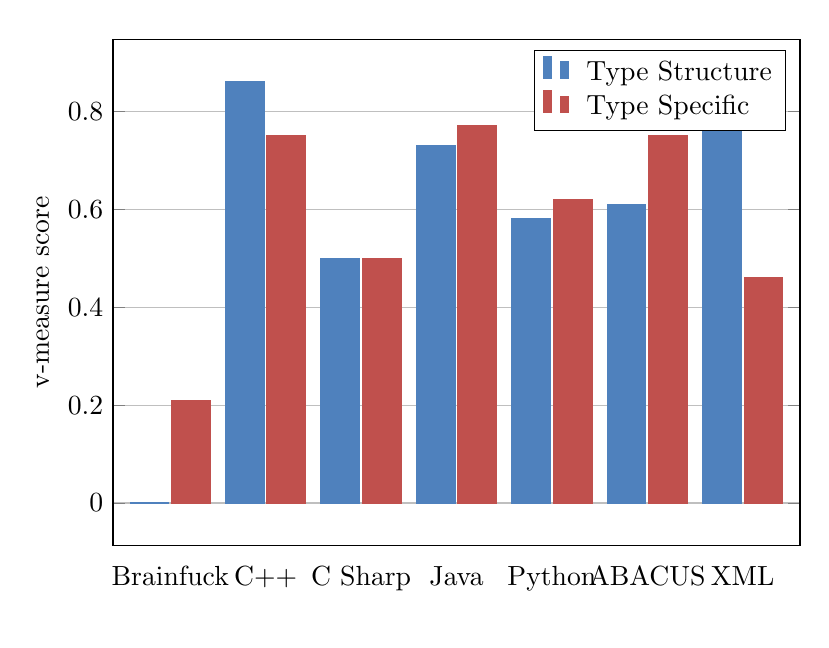
\begin{tikzpicture}
\begin{axis}[
width  = 0.85*\textwidth,
height = 8cm,
major x tick style = transparent,
ybar=1pt,
legend cell align=left,
legend style={ column sep=1ex },
bar width=14pt,
ymajorgrids = true,
ylabel = {v-measure score},
symbolic x coords={Brainfuck,C++,C Sharp, Java,Python,ABACUS,XML},
xtick = data,
scaled y ticks = false,
]
\addplot[style={bblue,fill=bblue,mark=none}]
coordinates {(Brainfuck, 0) (C++,0.86) (C Sharp,0.5) (Java, 0.73) (Python,0.58) (ABACUS,0.61) (XML,0.77)};

\addplot[style={rred,fill=rred,mark=none}]
coordinates {(Brainfuck, 0.21) (C++,0.75) (C Sharp,0.5) (Java, 0.77) (Python,0.62) (ABACUS,0.75) (XML,0.46)};

\legend{Type Structure,Type Specific}
\end{axis}
\end{tikzpicture}
For Java it was clear that only the Type Representers worked well. Weight Summary could improve the results, but was not guaranteed to. For evaluating which of the two Type Representers performs better, we calculated v-measure scores for both Type Representers on 6 additional Languages.
It is hard to see, which one of the two Type Representers does overall perform better, as their performance relies heavily on the input. This also stands out if we calculate the averages of all the scores of the Type Structure and Type Specific representation. The average of all scores of the Type Structure Representer is $0.57$, while the average of all the Type Specific representation lies by $0.58$. But if we look at the average of the best performed representations per language, we get a score of $0.64$, and if we ignore Brainfuck, which we were not good in clustering it at all, we get a score of $0.71$. This makes it hard to tell, which of the two Representers is overall expected to perform better, as scores depend more on input language as on the Representer. Predictions based on the languages are very hard. As we saw in this chapter, even closely related languages can behave very differently in the clustering process.

\section{Applicability for other languages}\label{sec:evaluating-other-languages}
The main evaluation of the k-means algorithm was done for Java. As a result of section \ref{sec:v-measure-scores-for-java}, we can now discard certain representations as not suitable. We will now take a look at the performance of the representations for other languages than Java, including an Abacus \cite{abacus2016} log file, for evaluating how our tool varies for different languages. It is desirable that it performs well on other languages, because we want StructureFinder to be able to cluster unknown languages reasonably. All the input files used for clustering contain source code randomly selected from Github. Each file contains roughly about 300 lines of code or more from different source files.
\subsection{C\#}
\begin{table}[H]
	\begin{center}
		\caption{C Sharp v-measures}
		\label{table1}
		\pgfplotstabletypeset[
		%trim cells,
		%multicolumn names, % allows to have multicolumn names
		col sep=semicolon, % the seperator in our .csv file
		read comma as period=true,
		%column type=1,
		precision =2,
		every head row/.style={%
			before row=\toprule,
			after row=\midrule,
			typeset cell/.code={
				\ifnum\pgfplotstablecol=\pgfplotstablecols
				\pgfkeyssetvalue{/pgfplots/table/@cell content}{\multicolumn{1}{c}{##1}\\}%
				\else
				\pgfkeyssetvalue{/pgfplots/table/@cell content}{\multicolumn{1}{c}{##1}&}%
				\fi
			}
		},
		every last row/.style={after row=\bottomrule},
		display columns/0/.style={string type,column type={l}},
		display columns/1/.style={string type},
		display columns/2/.style={string type},
		display columns/3/.style={string type},
		display columns/4/.style={string type},
		display columns/5/.style={string type},
		]{vmeasures/vmeasurescsharp.csv} % filename/path to file
	\end{center}
\end{table}
If we look at the taxonomy of programming languages, we see that C\# is very close to Java. Therefore, it is to be expected that many structural elements are the same for both languages. It is not a surprise that the results of our methods are not that different to those calculated for Java. The heuristic for k is not as good as for Java. While we manually classified C\# into 17 clusters, even the best guess missed two clusters. This makes $\alpha = -3$ not the best choice for C\#. Nevertheless, the scores for the single use of the Type Representers are satisfying with the best v-measure around $0.8$. But it stands out, that the Weight Summary Representer - our noise reduction - does not perform as good as in Java. This is surprising, given the close relation between Java and  C\#. While it resulted in good scores for Java, giving the best score with Type Specific representation, the scores for C\# are remarkably low. Differences can lie in the composition of the used data. For this thesis around 300 lines of code for each language are used in the clustering of the language. A big challenge in clustering is the correct assignment of comments. If a code contains lots of comments that are formatted in different ways or even software code that is commented out, this will be clustered differently from intended. The C\# code used for clustering shows indeed lots of different comments, that were not clustered as intended.

It is also surprising, that we have way more empty centroids than in Java. The clustering of Java resulted in neither of the used representations used for C\# in empty centroids. It is not clear as to why this happens. One thing that seems to be standing out, is that the use of the noise reduction, in general either improves the result, or causes it to have more empty centroids. This can be the case because reducing noise also means that information is removed, lowering the dimension of the vectors. If too much information is removed, the clustering cannot work properly, as variance of the data may become too low, so that data points cannot be distinguished well enough.
\subsection{C++}
\begin{table}[H]
	\begin{center}
		\caption{C++ v-measures}
		\label{table1}
		\pgfplotstabletypeset[
		%trim cells,
		%multicolumn names, % allows to have multicolumn names
		col sep=semicolon, % the seperator in our .csv file
		read comma as period=true,
		%column type=1,
		precision =2,
		every head row/.style={%
			before row=\toprule,
			after row=\midrule,
			typeset cell/.code={
				\ifnum\pgfplotstablecol=\pgfplotstablecols
				\pgfkeyssetvalue{/pgfplots/table/@cell content}{\multicolumn{1}{c}{##1}\\}%
				\else
				\pgfkeyssetvalue{/pgfplots/table/@cell content}{\multicolumn{1}{c}{##1}&}%
				\fi
			}
		},
		every last row/.style={after row=\bottomrule},
		display columns/0/.style={string type,column type={l}},
		display columns/1/.style={string type},
		display columns/2/.style={string type},
		display columns/3/.style={string type},
		display columns/4/.style={string type},
		display columns/5/.style={string type},
		]{vmeasures/vmeasurescpp.csv} % filename/path to file
	\end{center}
\end{table}
C++, like C\#, is very closely related to Java. So similar results are to be expected. With Type Structure and Type Specific representation, this is the case, even though they score lower. It is suspected, that there are the same problems in clustering, as in C\#. C++ does also contain different ways for commenting, that are difficult to handle. The scores of C++ are more similar to C\# than to those calculated for Java.\\\\
Like C\#, the manual clustered example contained 17 clusters. The number of clusters, was guessed better than for C\#. With Type Structure and Type Specific only missing one cluster and Type Specific with applied Weight Summary guessing the correct k.
\subsection{Phyton}
\begin{table}[H]
	\begin{center}
		\caption{Phyton v-measures}
		\label{table1}
		\pgfplotstabletypeset[
		%trim cells,
		%multicolumn names, % allows to have multicolumn names
		col sep=semicolon, % the seperator in our .csv file
		read comma as period=true,
		%column type=1,
		precision =2,
		every head row/.style={%
			before row=\toprule,
			after row=\midrule,
			typeset cell/.code={
				\ifnum\pgfplotstablecol=\pgfplotstablecols
				\pgfkeyssetvalue{/pgfplots/table/@cell content}{\multicolumn{1}{c}{##1}\\}%
				\else
				\pgfkeyssetvalue{/pgfplots/table/@cell content}{\multicolumn{1}{c}{##1}&}%
				\fi
			}
		},
		every last row/.style={after row=\bottomrule},
		display columns/0/.style={string type,column type={l}},
		display columns/1/.style={string type},
		display columns/2/.style={string type},
		display columns/3/.style={string type},
		display columns/4/.style={string type},
		display columns/5/.style={string type},
		]{vmeasures/vmeasuresphyton.csv} % filename/path to file
	\end{center}
\end{table}

Python does have similar constructs as Java, but is not as closely related to it compared to C++ or C\#. The evaluation of Python shows reasonable clusterings for Type Structure and Type Specific, but does also not well, if Weight Summary representation is applied. If we include the guessed value for k and the number of centroids, Type Structure does better than Type Specific representation, even though the Type Specific alone does have a higher score. Unfortunately, k is not guessed as well for Type Structure as for Type Specific. The number of clusters in our manually created clustering is 12. Elbowing does achieve a good value for the Type Structure Representer, with or without the application of Weight Summary Representer, creating only one extra cluster. For Type Specific, k is guessed to big, having 4, respectively 6 additional clusters than the manually created clustering. If we take a look at the used code, we see lots of different statements beginning with "print" and should be assigned to the same cluster. Having just one word at the beginning of the statement characterising the whole statement works the same way as comments do. This makes it hard for the clustering algorithm to assign them properly.
\subsection{XML}
\begin{table}[H]
	\begin{center}
		\caption{XML v-measures}
		\label{table1}
		\pgfplotstabletypeset[
		%trim cells,
		%multicolumn names, % allows to have multicolumn names
		col sep=semicolon, % the seperator in our .csv file
		read comma as period=true,
		%column type=1,
		precision =2,
		every head row/.style={%
			before row=\toprule,
			after row=\midrule,
			typeset cell/.code={
				\ifnum\pgfplotstablecol=\pgfplotstablecols
				\pgfkeyssetvalue{/pgfplots/table/@cell content}{\multicolumn{1}{c}{##1}\\}%
				\else
				\pgfkeyssetvalue{/pgfplots/table/@cell content}{\multicolumn{1}{c}{##1}&}%
				\fi
			}
		},
		every last row/.style={after row=\bottomrule},
		display columns/0/.style={string type,column type={l}},
		display columns/1/.style={string type},
		display columns/2/.style={string type},
		display columns/3/.style={string type},
		display columns/4/.style={string type},
		display columns/5/.style={string type},
		]{vmeasures/vmeasuresxml.csv} % filename/path to file
	\end{center}
\end{table}

All the previously evaluated programming languages have similar constructs. This cannot be said about XML, as it is a hierarchical mark-up language. The best results were scored with the Type Structure Representer, scoring high in homogeneity and completeness. The other results are not conclusive, because it cannot be determined, if noise reduction does help or not.

The manually clustered example contains 15 clusters. This means, that for XML, the elbowing parameter $\alpha = -3$ does not seem to be the best choice, as the guess for k is too low over all the evaluated representations.
\subsection{ABACUS log file}
\begin{table}[H]
	\begin{center}
		\caption{ABACUS log v-measures}
		\label{table1}
		\pgfplotstabletypeset[
		%trim cells,
		%multicolumn names, % allows to have multicolumn names
		col sep=semicolon, % the seperator in our .csv file
		read comma as period=true,
		%column type=1,
		precision =2,
		every head row/.style={%
			before row=\toprule,
			after row=\midrule,
			typeset cell/.code={
				\ifnum\pgfplotstablecol=\pgfplotstablecols
				\pgfkeyssetvalue{/pgfplots/table/@cell content}{\multicolumn{1}{c}{##1}\\}%
				\else
				\pgfkeyssetvalue{/pgfplots/table/@cell content}{\multicolumn{1}{c}{##1}&}%
				\fi
			}
		},
		every last row/.style={after row=\bottomrule},
		display columns/0/.style={string type,column type={l}},
		display columns/1/.style={string type},
		display columns/2/.style={string type},
		display columns/3/.style={string type},
		display columns/4/.style={string type},
		display columns/5/.style={string type},
		]{vmeasures/vmeasureslog.csv} % filename/path to file
	\end{center}
\end{table}
The ABACUS log files does achieve good scores, even though there are many empty centroids in the final clusterings. Only one representation methods has a score lower than $0.5$. In the scores gathered, it stands out, that Weight Summary representation only improves the score, if used with Type Specific representation. For Type Structure Representer this does not apply. The number of clusters would have been guessed pretty good by the elbow method. But if we subtract the empty centroids from it, we get too few clusters.

It is not certain, why the clustering of the ABACUS log files results in this many empty centroids, but it could mean that there is a lot of the same types in the same part of the statements, causing problems with the initialization of the centroids, as was discussed before. The problem with this explanation is, that Type Structure with Weight Summary does no perform better, which should be expected in that case.
\subsection{Brainfuck}
\begin{table}[H]
	\begin{center}
		\caption{Brainfuck v-measures}
		\label{table1}
		\pgfplotstabletypeset[
		%trim cells,
		%multicolumn names, % allows to have multicolumn names
		col sep=semicolon, % the seperator in our .csv file
		read comma as period=true,
		%column type=1,
		precision =2,
		every head row/.style={%
			before row=\toprule,
			after row=\midrule,
			typeset cell/.code={
				\ifnum\pgfplotstablecol=\pgfplotstablecols
				\pgfkeyssetvalue{/pgfplots/table/@cell content}{\multicolumn{1}{c}{##1}\\}%
				\else
				\pgfkeyssetvalue{/pgfplots/table/@cell content}{\multicolumn{1}{c}{##1}&}%
				\fi
			}
		},
		every last row/.style={after row=\bottomrule},
		display columns/0/.style={string type,column type={l}},
		display columns/1/.style={string type},
		display columns/2/.style={string type},
		display columns/3/.style={string type},
		display columns/4/.style={string type},
		display columns/5/.style={string type},
		]{vmeasures/vmeasuresbrainfuck.csv} % filename/path to file
	\end{center}
\end{table}
Brainfuck differs from any other programming language evaluated in this thesis. Brainfuck uses only eight different special characters as instructions, with everything else being treated as comments. This makes clustering the statements very hard, as there is very little difference between statements. Even though we remarked in the evaluation of Java that fewer variance can result in better scores, it is clear that too low variance cannot be clustered correctly, as all statement representation vectors gather around the same points. Because we initialize centroids uniformly over all dimensions, this results in many empty centroids for Brainfuck. Also, it is important to see, that noise reduction goes awry as well. Noise reduction reducing the dimension of the representations remarkably, because Brainfuck only uses one type of tokens for all instructions. Reducing dimensions, does also mean that we loose information. This may work well for Java, as it really reduces noise, but in Brainfuck, it looses too much information to still be clustered correctly.
\subsection{Discussion}
We can see that StructureFinder can cluster different languages reasonably. For this we picked languages of which not all are closely related. This can help us anticipate if StructureFinder is able to cluster languages we do not have a lot of information about. And as discussed for each language clustered the results are satisfying. Nevertheless there are some problems that need to be addressed which can affect the clustering.

\textbf{Comments.} Comments are hard to find. In programming languages there is often, more than one way a comment can be defined, as well as the possibilities for using single-line or multi-line commenting. A comment is most of the time defined by the first few tokens in a statement, with the rest of the statement containing arbitrary structural information and sometimes even out-commented software code. This makes them very hard to cluster correctly.

\textbf{Formatting.} Our approach for creating statements (taking every new line as a statement, see section \ref{sec:statements-and-tokens}) is depended on the correct formatting of the software code. Not correctly formatted code can cause structure not being statementized correctly.

\textbf{Statements.} In StructureFinder, carriage return is the used delimiter for creating statements. This is a very simple approach and does not need to map the structure of loop based programming languages adequately.

\textbf{Dimensionality.} There are different dimensions in the data that need to be looked at: vector dimension, number of clusters expected and the number of lines in the input. If one of those mentioned dimension is too low, it can result in not proper clustering by the k-means algorithm, because it does not have enough difference in the data to assign them to different clusters. More dimension can contain more information. Low vector dimension could be causing the problems in clustering Brainfuck, as it contain almost only punctuation tokens.

\textbf{Summary.} Different Languages behave differently in our clustering approach. But with the exception of Brainfuck the v-measure scores for the clusterings are satisfying. It is unfortunately not possible at the moment to make predictions of how the composition of the language affects the outcome of the clustering algorithm, because related languages behave differently. This difference in behaviour could also be caused by the limited size of the input. It is important to note that the size of the input used for the evaluation was only around 300 lines of code each. Even though they were gathered from different source files, the results calculated in this thesis are purely experimental and do not allow for statistical conclusions on what to do or not to do in regards to the contents of the input. 

\section{Evaluation the Output}
If we take a look at the tables \ref{tab:measure-strcuture} and \ref{tab:measure-sec}, we can see that our calculated scores indicate that the clusterings made from StructureFinder to some extent matches our manually created clusterings. In this section we look now at the output of the tool -as described in section \ref{sec:kpipeline}- to find out, what we can learn from the nearest statements of the centroids and if these statements can help to gain an overview of the structure the languages used in our input files and thus help a developer in creating parser rules. For this we look at the nearest statements for Java input files, created using first, Type Structure Representer and second Type Specific Representer with elbow parameter $\alpha = -3$.
\begin{figure}[H]
	\centering
	\includegraphics[width=1\textwidth]{TypeStructureStatemetns.png}
	\caption{Nearest statements per centroids, created witch Type Structure Representer}
	\label{fig:typestructure}
\end{figure}
Each line of figure \ref{fig:typestructure} represents a centroid and with this the perfect example of the pattern a centroid should be composed of. Therefore it would be desired that these statements differ in their pattern. As though we can see different statements with different constructs in figure \ref{fig:typestructure}, there are multiple occurrences of similar statements. The first thing that stands out is the occurrence of two different lines which are related to commenting. It is clear that comments are problematic in our clustering approach, because the beginning of the statements and not the representation of the whole information defines the cluster it should be assigned to.
Also, there are two almost identical statements on line 1 and line 4 with the difference of one token. This means, that the length of the representation does play a big part in the assignments of the statements to clusters. It is to note here, that this would be the same statement, if Weight Summary Representer would have been used with the Type Structure Representer. Also we have two centroids declaring imports and two method declarations. Also interesting is to note what is missing. There are no conditionals (if) and no while or for loops in our generated figure \ref{fig:typestructure}. In our manual clustering we assigned all if statements to one centroid.

\begin{figure}[H]
	\centering
	\includegraphics[width=1\textwidth]{TypeSpecificStatemetns.png}
	\caption{Nearest statements per centroids, created witch Type Specific Representer}
	\label{fig:typespec}
\end{figure}

Type Structure Representer does a better job, assigning the comments to the same clusters. We still have the problem here that we have two nearly identical patterns, starting with the import token. It would be desired to have them assigned to the same cluster. The only difference of those two statements lies in the lengths of the statement and further more only in a series of a repeating pattern. It should clear that these two should be assigned to the same cluster. This is a huge draw back of our implemented approaches. Also we have the same problem as in figure \ref{fig:typestructure} above, here in line 3 and 4 in figure \ref{fig:typespec}, with statements that only differ in one word.

\subsection{Discussion}
It is possible to learn about key-constructs of the language clustered with StructureFinder. A problem is that there are different centroids with the same patterns as their nearest data point. This means that even though we have a good matching to our manually clustered example -as can be seen in the v-measure scores in section \ref{sec:v-measure-scores-for-java}- the centres of our clusters are not necessarily at the desired position. This limits the number of different constructs we can learn from our nearest statements. Also, since we limit our assumption on the language, we cannot say how much structural constructs are missing from the created list and so we never have a complete overview of the language using the nearest statements of the centroids. Alternatively, we could look at the complete feed of statements per centroid which is also saved. But it is not efficient to sort through the same number of lines of the input.
\section{Evaluating Language Differentiation}
\label{sec:language-differentiation}
After evaluation the k-means algorithm, we now take a look at the performance of our expansion for calculating a precision value for how close languages are related. For this we calculate a matrix containing all the precision values between pairs of languages.
But this does not make it possible to infer parser rules from the nearest statements of the clusters.
\begin{table}[H]
	\begin{center}
		\caption{Cross Language Differentiation}
		\label{table1}
		\pgfplotstabletypeset[
		%trim cells,
		%multicolumn names, % allows to have multicolumn names
		col sep=semicolon, % the seperator in our .csv file
		read comma as period=true,
		%column type=1,
		precision =2,
		every head row/.style={%
			before row=\toprule,
			after row=\midrule,
			typeset cell/.code={
				\ifnum\pgfplotstablecol=\pgfplotstablecols
				\pgfkeyssetvalue{/pgfplots/table/@cell content}{\multicolumn{1}{c}{##1}\\}%
				\else
				\pgfkeyssetvalue{/pgfplots/table/@cell content}{\multicolumn{1}{c}{##1}&}%
				\fi
			}
		},
		every last row/.style={after row=\bottomrule},
		display columns/0/.style={string type,column type={l}},
		display columns/1/.style={string type},
		display columns/2/.style={string type},
		display columns/3/.style={string type},
		display columns/4/.style={string type},
		display columns/5/.style={string type},
		]{langdiff.csv} % filename/path to file
	\end{center}
\end{table}

The results of the Language Differentiator are unfortunately not as expected. 
It was expected that languages, like Java and C Sharp would be similar, because they both are a C type language, as are C++ and Python. But it was not expected, that nearly all values calculated, resulted near or are one. This applies also to the abacus log file, which is not even a language.
It would not suffice just to reference to the problems mentioned in section \ref{sec:explaining-the-results}. There must be a general flaw in the idea. \\\\
The underlying idea of the Language Differentiator was, that if we can cluster statements in a satisfying way, clusters of different statements in a single language would need to be further apart from statements of other clusters than from statements of the same cluster. The conclusion from this was, that different languages would result in different clusterings, with different centroids.

\textbf{Overlap.} While it is not possible in k-means, that clusters overlap. But it is possible for clusters of two languages to overlap, because they are created independently. If the variance of the data is small, then all data points of the statement representation of the two different languages are located in the same space. Therefore, if this is the case, our way of calculating language differentiation would not be able to find differences between the languages, because they would count as positive findings in our calculations.\\\\
This can be visualized in a two dimensional example.
\begin{figure}[H]
	\centering
	\includegraphics[width=0.8\textwidth]{circlesoverlap.pdf}
	\caption{Overlap of clusters in Language Differentiator}
	\label{fig:langdiffoverlapp}
\end{figure}
The orange, blue and red crosses visualize the vector points of the representation of the first language and the black circles are spanned from the radii from the centroids to the point of the cluster with longest distance. The green crosses, visualize the same for the second language. It is clear that these languages are not a close match, because the green crosses are divided to all three clusters created from the first language. But because the variance of the clusters is low, it is possible that all the green crosses lie in the radii of the clusters of the first language. This gives us for this example a precision value of $1$, even though if we would span a circle around the green crosses, it would intersect with all three circles spanned from the first language. A better approach for language differentiation with k-means could be to calculate a precision value not based on the vector data points, but on the centroids of the clustering of the second language.

\chapter{Conclusions and Future Work}
Finding structural patterns in code or log files can help infer grammar rules, as an important part of building a parser. In this thesis we introduce pattern recognition, using the unsupervised learning algorithm k-means and presented ways for representing the data for the used algorithm. Our goal was to minimize assumptions on the input, therefore allowing StructureFinder to work on any given code or log files.
We evaluated these method to see if they perform as expected.

Representations were calculated using different representation, which can be chained together, using one Representer of each category, categorized in Type Representers, Distance Representers and Weight Representers.

The evaluation of the representations indicate, that using Type representations without any other representation performs best for almost all. Using Weight Summary representation for noise reduction can further improve the results on some languages, but is not guaranteed to perform better. If we take a better look at the Type Representers, Type Specific does perform slightly better for any tested language.

Apart from the results given by the Type Representers and/or Weight Summary representation, the other representations did not do well in the evaluation, having low scores and were not robust regarding their computations, having high variance in multiple runs and resulting in empty centroids.

If we look at the centroids and the nearest statements located to those centroids, we have an overview of different structures of the clustered language. Unfortunately, despite good v-measure scores it is possible to have statements, who we manually assigned to the same clusters, featured as nearest statements of two different centroids. Nevertheless, key features of the language can be identified, but it is not possible to know what patterns are not featured in this list of statements. This gives us no complete overview of the language and makes it hard to infer parser rules from the nearest statements.

In this thesis it stands out that k-means for clustering structural patterns in code clearly has limitations, as k-means itself does make assumptions on the data while clustering, as it always tries to find circular shaped clusters.

Our introduced approach for calculating how closely related languages are did not perform well. It resulted almost in every case in a precision value of one. Meaning that both languages should be the same.

\section{Future Work}
Regarding the Problems of k-means, different unsupervised learning algorithms, using single linkage or hierarchical clustering work better for certain languages, as they make different assumptions regarding their input.

The execution of the k-means implementation is quite expensive for big data sets and in particular, if the vectors contain floating point numbers. Better implementation of vector computations could certainly improve the run time of our tool.

In this thesis, the main focus lies on the different representations and the implementation of the k-means pipeline. The statements were created as single lines, as we wanted to limit our assumptions. Most programming languages have block structures, allowing for encapsulating their statements. The new line approach does not allow for encapsulation. Improvement on the creation of statements could improve the quality of the output of StructureFinder.

With the knowledge about the assumption made by the k-means algorithm, we could also try to make more representations, which could exploit those assumptions better.

It would also be interesting to see, how the results could be improved, if we add heuristics for finding keywords. Keywords are a very important construct of programming languages, that cannot be found with our representation approach. Comments or print statements can add different structure after a keyword, but should be assigned to the same cluster. Adding information about keywords, for example as a forth type for tokens, could improve the clusterings.

For language differentiation the approach could be changed to calculate the precision value based on the centroid of a cluster and not on the statements representation vector points of a language. This could reduce the problem of the general overlap of data with low variance. 
\listoftables
\lstlistoflistings
\listoffigures
\bibliography{thesis}
\bibliographystyle{plain}
\chapter{Anleitung zu wissenschaftlichen Arbeiten}
This chapter contains additional documentation for the StructureFinder tool, implemented in Pharo 4.0 and does also consist of a users guide to get the data, used in this thesis.
\section{Introduction}
The main effort in this bachelor thesis lies in the implementation of the clustering and representation mechanics. There are three different parts in our finished StructureFinder tool:

\begin{itemize}
	\item \textbf{StructureFinder.} Clusters the given input.
	\item \textbf{StructureAnalyzer.} Analysing mode of StructureFinder, clusters the input and returns additional information about how well it performed.
	\item \textbf{LanguageDifferentiator.} Expansion of StructureFinder, calculates a precision value for two input languages or can additional be used for cross comparison of different languages.
\end{itemize}

\section{Getting Started}
For replicating the results of this thesis or to play around with the clustering mechanics Pharo 4.0 and the used Image File in this thesis.\\\\
Pharo 4.0 with a standard Pharo 4.0 Image can be downloaded from:\\\\
\textit{https://github.com/countschokula/BA\_StructurFinder}\\\\
The Image you need, containing the source code of this thesis is stored on a git repository and can be cloned using the git command:\\\\
\textit{\$ git clone https://github.com/countschokula/BA\_StructurFinder}


\section{Structure Finder}\label{sec:structure-finder}
The StructureFinder is the implemented k-means clustering tool.
For the execution, a folder structure needs to be created, containing the input files and folders for the output files. For proper functioning, the folder structure needs to look exactly like this. This needs to be manually created. If a new language is added, folders must be created in the folders files and result. "testFiles" is the root folder. In an input Folder there can be more than one file present. If that is the case, StructureFinder will concatenate them to one file in the clustering process.
\begin{figure}[H]
	\centering
	\label{fig:output}
	\includegraphics[width=0.8\textwidth]{folderStrFinder.png}
	\caption{Folder structure for setting up the StructureFinder tool, testFiles is the root folder}
\end{figure}
In the uploaded Image there should be preconfigured playgrounds. If there is no playground open, one needs to be opened.\\\\
The preconfigured playground for the StructureFinder contains all necessary parameters for running the clustering algorithm:
\begin{figure}[H]
	\centering
	\label{fig:playstruct}
	\includegraphics[width=1\textwidth]{strFinderPlayground.png}
	\caption{Pharo 4.0 playground for configuring and running StructureFinder}
\end{figure}
For better understanding, the preconfigured playgrounds contains information on the parameters, that can be set. We now take a closer look at the parameters of the StructureFinder.
\begin{itemize}
	\item \textbf{path.} This parameter is necessary for correct loading and storing of the input respectively the output files. The path should point to the root of the folder structure as defined above.
	\item \textbf{mode} It is possible to run two different modes of StructureFinder. Parameter "1" creates a single run of the clustering for input k, while parameter "2" runs the clustering for every natural number between k2 and k.
	\item \textbf{inputFolder.} It is possible to have different folders, containing different languages in your project root folder. The message "inputFolder:" makes the tool use the input of the folder. The folder is given as a string. Output is saved in the corresponding folder under results.
	\item \textbf{k.} Number of clusters for single clustering. If interval mode is activated, k is the higher limit of the interval.
	\item \textbf{kmin.} If interval mode is activated, kmin is the lower limit of the interval.
	\item \textbf{iterations} Gives the kMeansRunner the number of iterations it should run the k-means algorithm, 25 is a low, fast and reasonably guess for the number of iteration. If no iteration value is set, the default value is 50.
	\item \textbf{$\alpha$.} Defines the threshold for the elbow method, the heuristic for guessing k. This parameter is only used, if the tool is run on an interval.   
	\item \textbf{typeRep.} A Type Representer must be set. Representers are given to the StructureFinder as Instances. There are two Type Representers available. TypeStructure and TypeSpecific.
	\item \textbf{distRep.} A Distance Representer is optional. It can be set by giving the StructureFinder an Instance of the Distance Representer you want to use. Currently there are two Distance Representers available. DistanceZero- and DistanceAllRepresenter.
	\item \textbf{weightRep.} Adding a Weight Representer is optional. Currently there are tree different Weight Representers available. WeightSummary-, WeightSum- First and WeightInverseRepresenter.
\end{itemize}
\textbf{Output.} The statements of a cluster are saved to .txt files. A file per centroid is created and the files are enumerated. They are saved under results in the corresponding folder the input file is located and are put in a folder named with the timestamp of the execution of the algorithm. For interval execution, for each created clustering the result will be saved:
\begin{figure}[H]
	\centering
	\label{fig:output.5}
	\includegraphics[width=1\textwidth]{outputfolder.png}
	\caption{Output Folders and Files under Windows}
\end{figure}
As seen in Figure \ref{fig:output.5} a file named configuration\_used will be created. It contains the parameters used in calculating the clusters, as well as the value of the distortion functions averaged over k, for all sets of clusters. Also, the nearest statements to the centroids are listed.
\begin{figure}[H]
	\centering
	\label{fig:output2}
	\includegraphics[width=1\textwidth]{logOutput.png}
	\caption{Example of "configuration\_used.txt" log file.}
\end{figure}
\section{Structure Analyzer}
Structure Analyzer allows for calculating the v-measure scores. V-measure is explained in detail in section \ref{sec:v-measures}. \\\\
For calculating v-measures, it is necessary to have a manually created clustering of your input data to test against. The input file needs to be split into the clusterings wanted to be achieved and saved into different text files. The assigned statements must be only featured once in the manually created clusters. Also, the cluster set must be stored in the correct folder. For this a folder named "perfect" needs to be created in the root folder of your project path. In the folder "perfect" a folder with the same name as the input folder has to be created and this is were the manually assigned clusters need to be stored. The input of the files has to be on the same location used for the StructureFinder.

\begin{figure}[H]
	\centering
	\label{fig:output3}
	\includegraphics[width=1\textwidth]{folderPerfect.png}
	\caption{Set up of perfect example for analysing}
\end{figure}
 The configuration is exactly the same as in section \ref{sec:structure-finder} for the StructureFinder.\\\\
The preconfigured playground for the StructureAnalyzer looks like this:
\begin{figure}[H]
	\centering
	\label{fig:stAnPl}
	\includegraphics[width=1\textwidth]{strAnalyzerPlayground.png}
	\caption{Preconfigured StructureAnalyzer Playground}
\end{figure}

\textbf{Output} The StructureAnalyzer has the same output as the StructureFinder in section \ref{sec:structure-finder}. The exception is, that the additional information about the performance of the clusterings are added to the log file.
\begin{figure}[H]
	\centering
	\label{fig:lgOA}
	\includegraphics[width=1\textwidth]{logOutAna.png}
	\caption{Log file "configuration\_used", added performance information from analysation.}
\end{figure}
\section{Language Differentiator}
There are two different ways for calculating the Language Differentiator values. The first way, calculates the precision value of how close two languages are related, using two normal input files from the files directory, as described in section \ref{sec:structure-finder}. The second approach, which was used for calculating the results in this thesis, as can be found in section \ref{sec:structure-finder}, uses a different test and trainings set per language, allowing to test the relation of two different input sets for the same language.\\\\
We now take a look at the first approach and the preconfigured Pharo playground.
\begin{figure}[H]
	\centering
	\label{fig:lgOA2}
	\includegraphics[width=1\textwidth]{ldiffPlayground.png}
	\caption{Language Differentiator Playground}
\end{figure}
The initialization of the LanguageDifferentiator works nearly the same as for the StructureFinder and the StructureAnalyzer. The exception is, that the kMeansRunner Object is not wrapped in the LanguageDifferentiator and must be initialised separately.\\\\
\textbf{Output.} For the playground to show the results, press Ctrl+A and Crtl+P. The clusters are saved in the normal result folder.\\\\
The second approach needs a separate folder structure:
\begin{figure}[H]
	\centering
	\label{fig:lgOA3}
	\includegraphics[width=1\textwidth]{compareFolderStr.png}
	\caption{Language Differentiator compare folder structure}
\end{figure}
There is also a preconfigured playground for the "crossLanguageComparison:"
\begin{figure}[H]
	\centering
	\label{fig:lgOA4}
	\includegraphics[width=1\textwidth]{crossPlayground.png}
	\caption{Language Differentiator cross comparison}
\end{figure}
The KMeansRunner is configured in the same way as above. All the folders that we want to compare with each other can be added in string form to the types collection with the message "add:".\\\\
\textbf{Output.} Output is generated using the playground command Ctrl+P. Results of the clusterings are saved to the results folder in compare>training>result.\\\\
%END Doc
%-------------------------------------------------------



\end{document}